
\subsection{Memcached Performance}
\label{sec:eval:memcached}



%FIXME if different keys


\begin{figure*}[t]

\centering
  \vspace*{0.3in}
 \subfloat[Throughput for varying established connections]{
  \label{fig:connscaling:throughput}
   
\includegraphics[width=.49\textwidth,clip]{figs/blank.eps}}
 \hspace{.02in}
 \subfloat[Avg. and 99\% latency for varying established connections]{
  \label{fig:connscaling:lat}
  
\includegraphics[width=.49\textwidth,clip]{figs/blank.eps}}
\centering
  \vspace{-2.8in}
  \subfloat{
\includegraphics[width=1\textwidth,clip]{figs/short-key.eps}}
 \vspace{2.3in}
 \
\caption{Connection scaling}
 \label{fig:connscaling}

\end{figure*}

\begin{figure*}
\begin{centering}
\subfloat[Latency vs throughput for the memcached ETC workload.]{
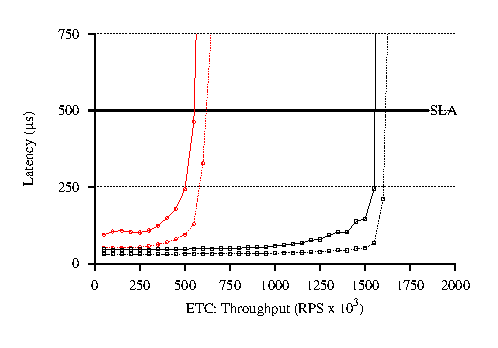
\includegraphics{figs/memcached-etc-basic.eps}}
\subfloat[Multilate-Me Again!]{

\includegraphics{figs/blank.eps}}
\caption{Capacity and quality of service of memcached on Linux and \ix for XXX and YYY concurrent, established connections}
\label{fig:mutilate}
\end{centering}
\end{figure*}



Finally, we evaluated the performance benefits of the \ix with
\texttt{memcached}, a widely deployed, in-memory key-value store built
on top of the \texttt{libevent} framework~\cite{url:memcached}. It is
frequently used as a high-throughput, low-latency caching tier in
front of persistent database servers. \texttt{memcached} is a
network-bound application, with threads spending over 80\% of
execution time in kernel mode for network
processing~\cite{DBLP:conf/eurosys/LeverichK14}. It is a difficult
application to scale because the common deployments involve high
connection counts for \texttt{memcached} servers and small-sized
requests and
replies~\cite{DBLP:conf/nsdi/NishtalaFGKLLMPPSSTV13,Atikoglu:2012:WAL}

We use the \texttt{mutilate} load-generator to place a selected load
on the server in terms of requests per second (RPS) and measure
response latency~\cite{url:mutilate}. \texttt{mutilate} coordinates a
large number of client threads across multiple machines to generate
the desired RPS load, while a separate unloaded client measures
latency by issuing one request at the time.  We configure
\texttt{mutilate} to generate load representative of two workloads
from Facebook~\cite{Atikoglu:2012:WAL}: the ETC workload that
represents that highest capacity deployment in Facebook, has 20B - 70B
keys, 1B-1KB values, and 75\% GET requests; and the USR workload that
represents deployment with most GET requests in Facebook, has short
keys ($<$20B), 2B values, and 99\% GET requests. In USR, almost all
traffic involves minimum-sized TCP packets. Each request is issued
separately (no \texttt{multiget} operations). However, clients
pipeline requests by up to a maximum of four outstanding requests per
connection. We use 16 client machines to generate load for a total of
276 connections to the memcached server.

To provide insights into the full range of system behaviors, we report
average and 99th percentile latency as a function of the achieved
throughput. The 99th-ile latency captures tail latency issues and is
the most relevant metric for datacenter
applications~\cite{DBLP:journals/cacm/DeanB13}. Most commercial
\texttt{memcached} deployments provision each server so that the
99th-ile latency does not exceed 200\microsecond to 500\microsecond.
We carefully tune the Linux baseline setup according to the guidelines
in \cite{DBLP:conf/eurosys/LeverichK14}: we pin memcached threads,
configure interrupt-distribution based on thread-affinity, and tune
interrupt moderation thresholds. We believe that our baseline Linux
numbers are as tuned as possible for this hardware using the
open-source version of \texttt{memcached-1.4.18}. We report the
results for the server configuration that provides the best
performance: 8 cores with Linux, but only 6 with \ix.

Porting \texttt{memcached} to \ix primarily consisted of adapting it
to use our event library. In most cases, the port was straightforward,
replacing Linux and \texttt{libevent} function calls with their
equivalent versions in our API. \edb{We also replaced {\tt pthread}
  locks with simple spin-locks.}  We did yet not attempt to tune the
internal scalability of {\it memcached}~\cite{DBLP:conf/nsdi/FanAK13}
or to support zero-copy IO operations.

\christos{fix the QPS vs RPS issue: use only one. trim the graph to 500usec}


%%
%% see  figs/data/memcache-sla-qps.txt

%82.5  139.6  650K
%42.0  54.3   1320K  --> 2.03x     --> 2.0x
%79.6  136.8  580K
%37.7  44.5   1620K  -->  2.74519  --> 2.7x


\begin{table}[b]
%\vspace{-1em}
\begin{center}
\begin{small}
\begin{tabular}{|l|c|c|c|}
\hline
%Configuration &  \multicolumn{2}{|c|}{Unloaded latency} &  QPS for SLA:\\
Configuration &  Minimum latency &  RPS for SLA:\\
&  @99th pct &  $<500$\microsecond@99th pct\\
\hline
ETC-Linux & 93\microsecond & 500K\\
ETC-IX    & 46\microsecond & 1500K\\
\hline
USR-Linux & 84\microsecond & 450K\\
USR-IX    & 31\microsecond & 2150K\\

\hline
\end{tabular}
\caption{Unloaded latency and maximum RPS for a given service-level agreement for the memcache workloads \texttt{ETC} and \texttt{USR}.}
%\vspace*{-2em}
\label{tbl:mutilate}
\end{small}
\end{center}
\end{table}



Fig.~\ref{fig:mutilate} shows the throughput-latency curves for the
two \texttt{memcached} workloads for Linux and \ix, while
Table~\ref{tbl:mutilate} reports the unloaded, roundtrip latencies and
maximum request rate that meets a service-level agreement, both
measured at the 99th percentile.  \ix noticeably reduces the unloaded
latencies to roughly half.  Note that we use Linux clients for these
experiments; running \ix on clients should further reduce latency.

At high request rates, the distribution of CPU time shifts from being
$>80\%$ in the kernel with Linux to $<10\%$ with \ix. This allows \ix
to increase throughput by \data{2.0}{3.4} and \data{2.7}{4.7} for
\texttt{ETC} and \texttt{USR} respectively at a 500\microsecond tail
latency SLA.  The improvement for \texttt{ETC} is lower due to the
increased lock contention within the application itself, in particular
for \texttt{ETC}, which has a higher write frequency.  Lock contention
within application code is also the reason that \ix cannot provide
throughput improvements with more than 6 cores.


%
\subsection{Multi-tier Performance}

\edb{THIS IS A STRECH STRETCH GOAL} 

Evaluating the performance of a highly-scalable, multi-tier
environment in a lab environment is challenging on multiple fronts:
first, there are ---to the best of our knowledge--- no universally
accepted multi-tier benchmarks that involve key-value stores and in
general that are representative of web-scale applications.  Second,
most lab enviornments are orders of magnitude smaller than a
datacenter.

Therefore, we construct a simple, synthetic multi-tier benchmark that
mimics the behavior of a social application stored in an in-memory
key-value store.  The application is a simple \texttt{http} server
that returns the top-most recent update among a users list of friends.
The application server parses the http request to
get the userid, uses the user id to return a friends-list from a
key-value store, and then queries the key-value store individually for
each friend for the most recent value.  It then processes replies and
return the top-most entries.  In our experiments, we model a database
with $10^7$ million users, each with 100 friends. 

We scale the benchmark to model a cluster deployment with $\alpha$
client connections per application server, $\beta$ httpd and $\gamma$
memcached servers.  Keys are distributed uniformly between the
$\gamma$ servers.  We model a large-scale deployment with
$\alpha=10^5$, $\beta=10^4$ and $\gamma=10^4$ on a deployment that consists of 4
actual application servers and 1 memcached server (running on our
server hardware with 4x10GbE connectivity).  Each application server
runs \texttt{lighthttpd} with the application logic written directly
within the server, and maintains a distinct connection for each of the
$\alpha$ virtual clients and $\gamma$ virtual nodes.  The key-value store is
running \texttt{memcache} as described in \S\ref{sec:eval:memcache}.
We use the remaining 14 client machines to simulate $4 \times \alpha$
clients and the 19th client to measure the latency of the application.

Fig.~\ref{missing} reports the latency as a function of the
throughput, as determined by varying the client load.  We compare a
Linux baseline with one in which \ix is used to run both the
application server and the memcached server.  We note that the choice
of operating system on the application server determines the number of
concurrent connections. Indeed, because of the coherence-free
execution model, each application server needs to open a distinct TCP
flow to the same virtual node for each of its hardware threads.

\edb{OPTIMISTIC: } Fig.~\ref{missing} shows that \ix can saturate the
hardware connectivity.  Indeed, the bottlneck consits of the
communication 






